\section{Algorithms Applicable to Graphs}
\label{sec:algorithms}

Algorithms for analyzing pathways and networks have been placed  into three main categories by~\cite{Khatri2012}: \ac{ORA}, \ac{FCS}, and \ac{PT}.
\ac{ORA} often focuses on the number of differentially expressed genes present or absent in a gene set compared to chance, while \ac{FCS} is less susceptible to large effects and considers the aggregate of groups of small effects.
\ac{PT} finally considers the biological relations between members of the pathway during analysis.

\subsection{BEL Algorithms}
\label{subsec:bel_algorithms}

Furthermore, Martin \textit{et al.} made the distinction between methods that rely on the assumption that protein activities are correlated with their corresponding mRNAs' expression changes (forward reasoning) versus the effect that upstream controllers of mRNA expression have (backwards reasoning)~\cite{Martin2014}.
These algorithms have been developed for a wide variety of applications, data formats, and graph types.
While many are heterogeneous, below are the most notable algorithms specific to networks from knowledge assemblies encoded in BEL.

\subsubsection{Reverse Causal Reasoning}

Reverse causal reasoning (\ac{RCR}) is an approach to identify the upstream controllers of biological patterns measured in an experiment; often differential gene expression experiments between healthy and diseased patients.
First, large knowledge assemblies are dissected into smaller hypothesis networks with one upstream node with multiple outgoing causal relations to target nodes represented by the experimental data set.
Each hypothesis network is scored by its concordance between the observed up- and down-regulations of targets nodes to the sign of the causal relation and by its richness, or the explanatory power of the hypothesis network~\cite{Catlett2013}.
An example hypothesis network is shown in Figure~\ref{fig:rcr_schematic}.

\begin{figure}
\captionsetup{format=plain}
\makebox[\textwidth]{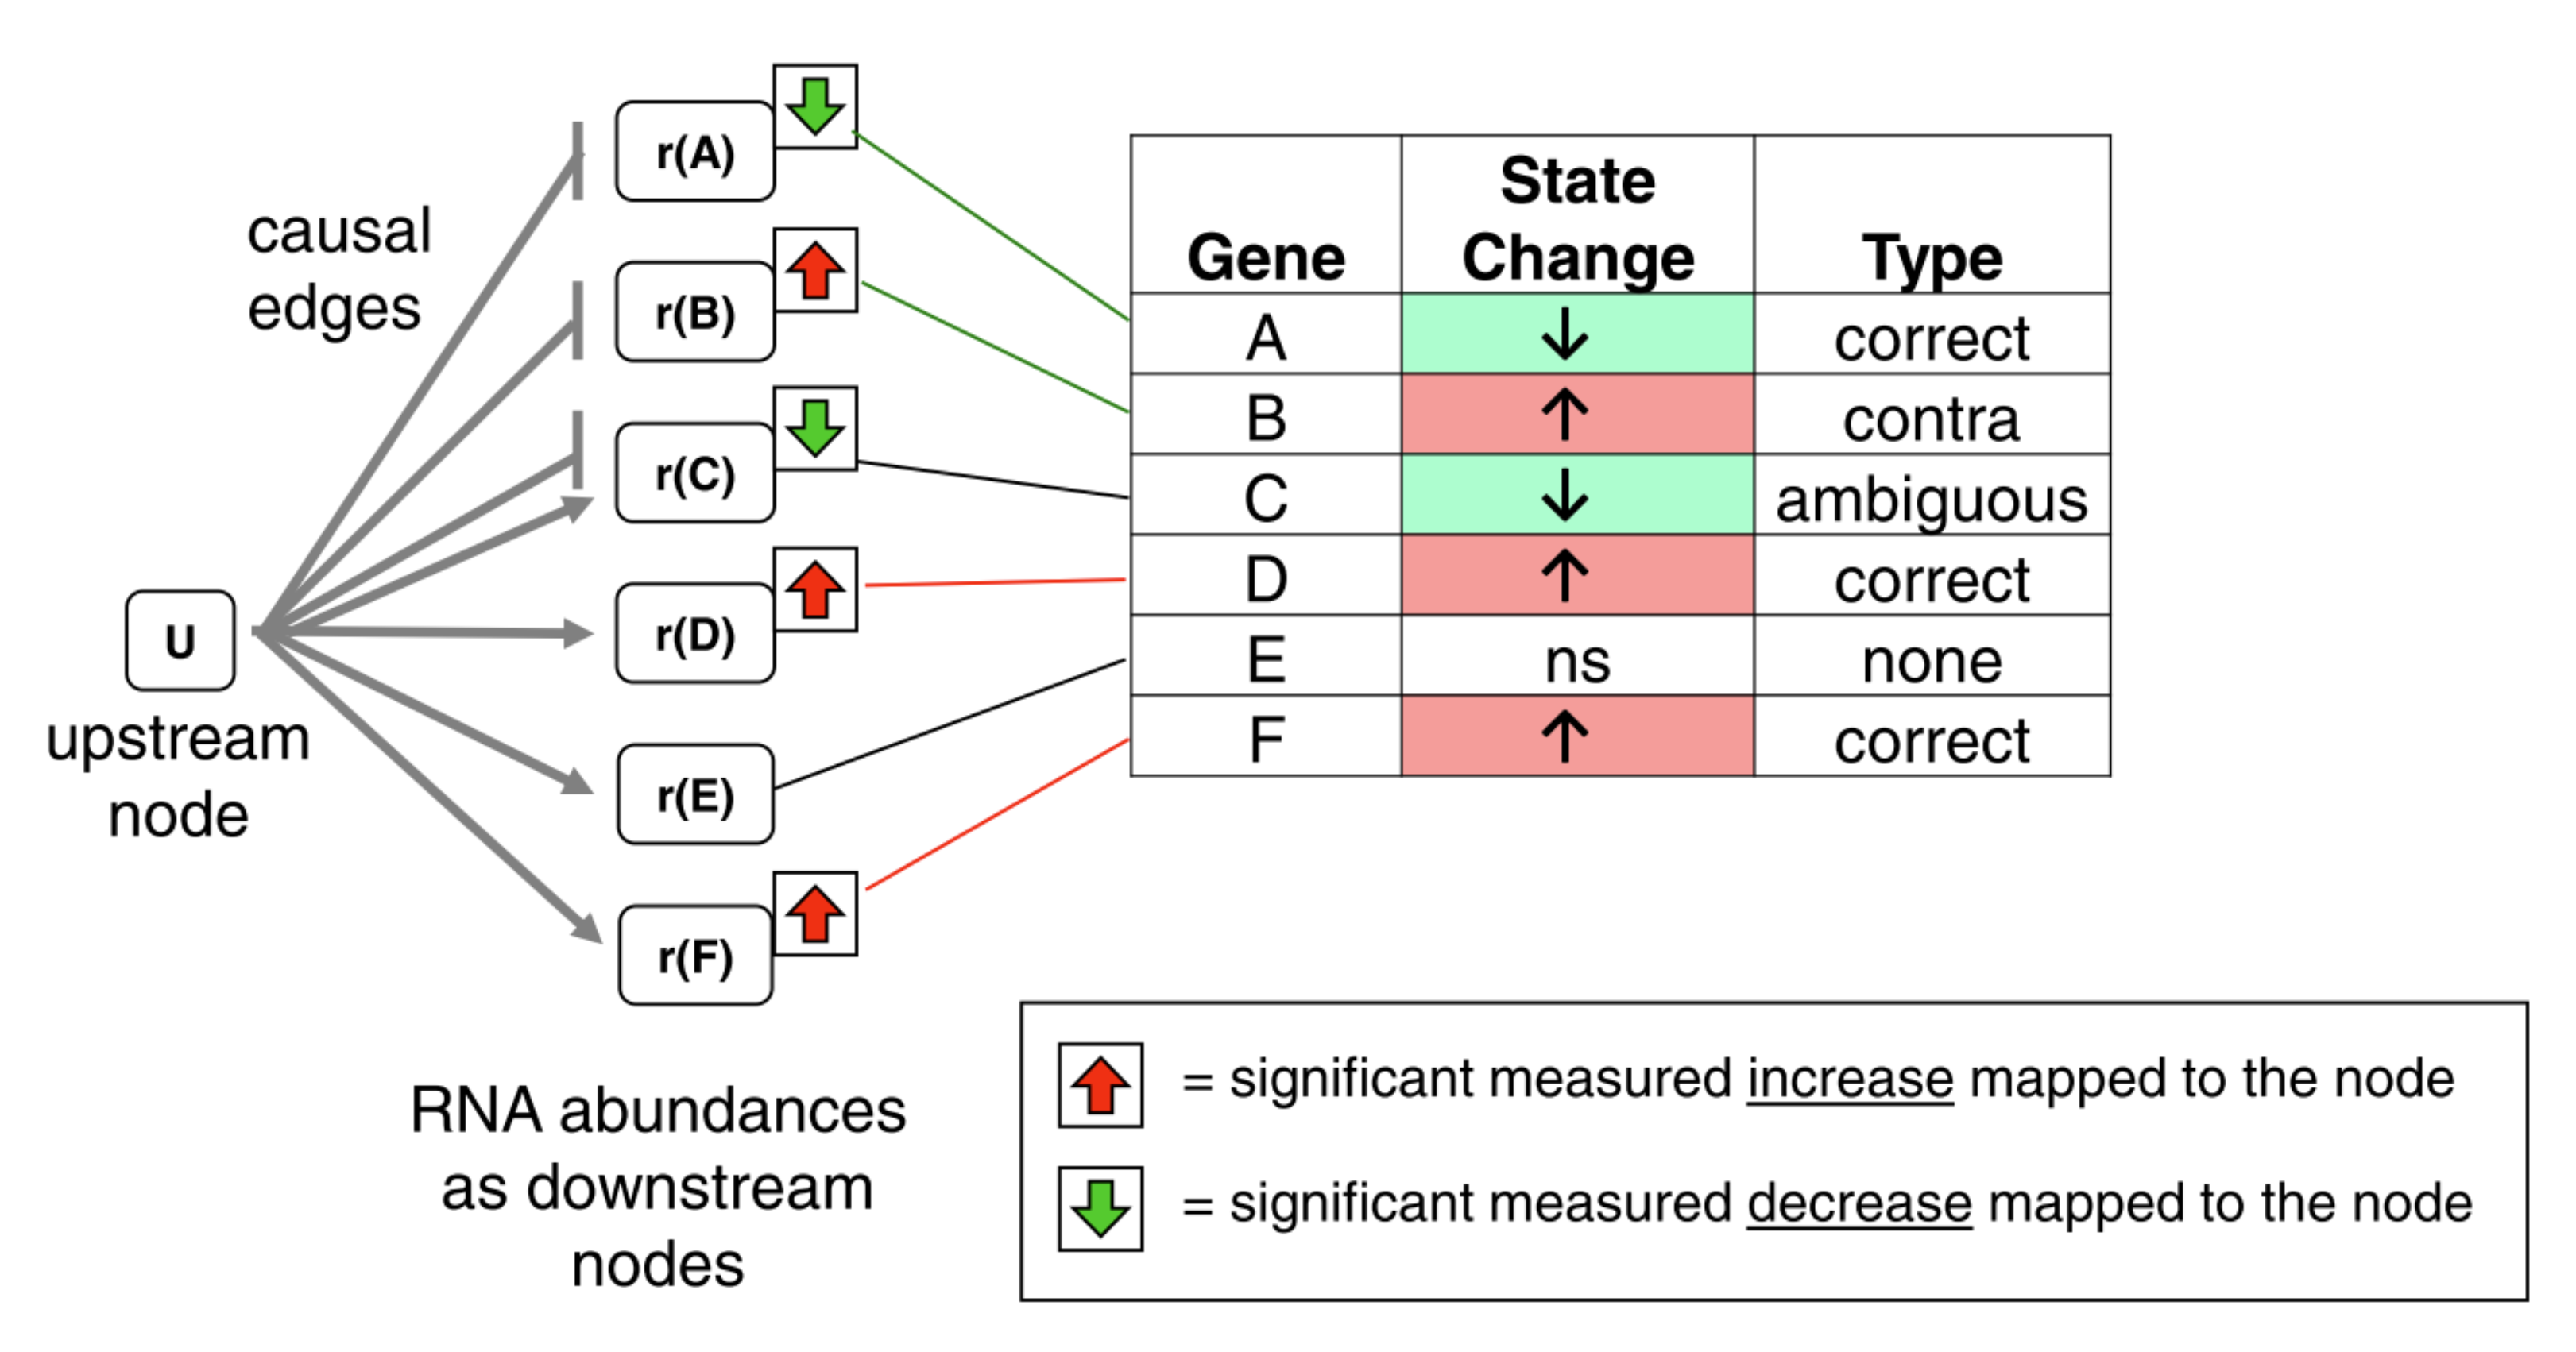
\includegraphics[width=160mm]{figures/rcr_schematic.png}}
\caption[A Schematic Diagram of \ac{RCR}]{An example hypothesis network. Target nodes are counted as correct if they have a decreasing relationship and down-regulation, or an increasing relationship and up-regulation. Target nodes with multiple conflicting relationships are marked as ambiguous. Finally, target nodes are counted as incorrect if they have a mismatch between an increasing relationship and down-regulation, or a decreasing relationship and up-regulation. Adapted from~\cite{Catlett2013}.}
\label{fig:rcr_schematic}
\end{figure}

\subsubsection{Network Perturbation Amplitude}

While \ac{RCR} gives preliminary insights to significant biological controllers, it mostly ignores the topology of signaling, regulatory, and other causal networks that can be represented in knowledge assemblies (Figure~\ref{fig:npa_schematic}).
The \ac{NPA} measures the aggregated effect explained by the controller layer with reference to a given node with respect to their downstream nodes.
Two complementary statistics for the effect of permutations of the upstream layer and downstream layer allow for further insight to the validity of \ac{NPA}s as a hypothesis generation mechanism~\cite{Martin2014}.

\begin{figure}
\captionsetup{format=plain}
\makebox[\textwidth]{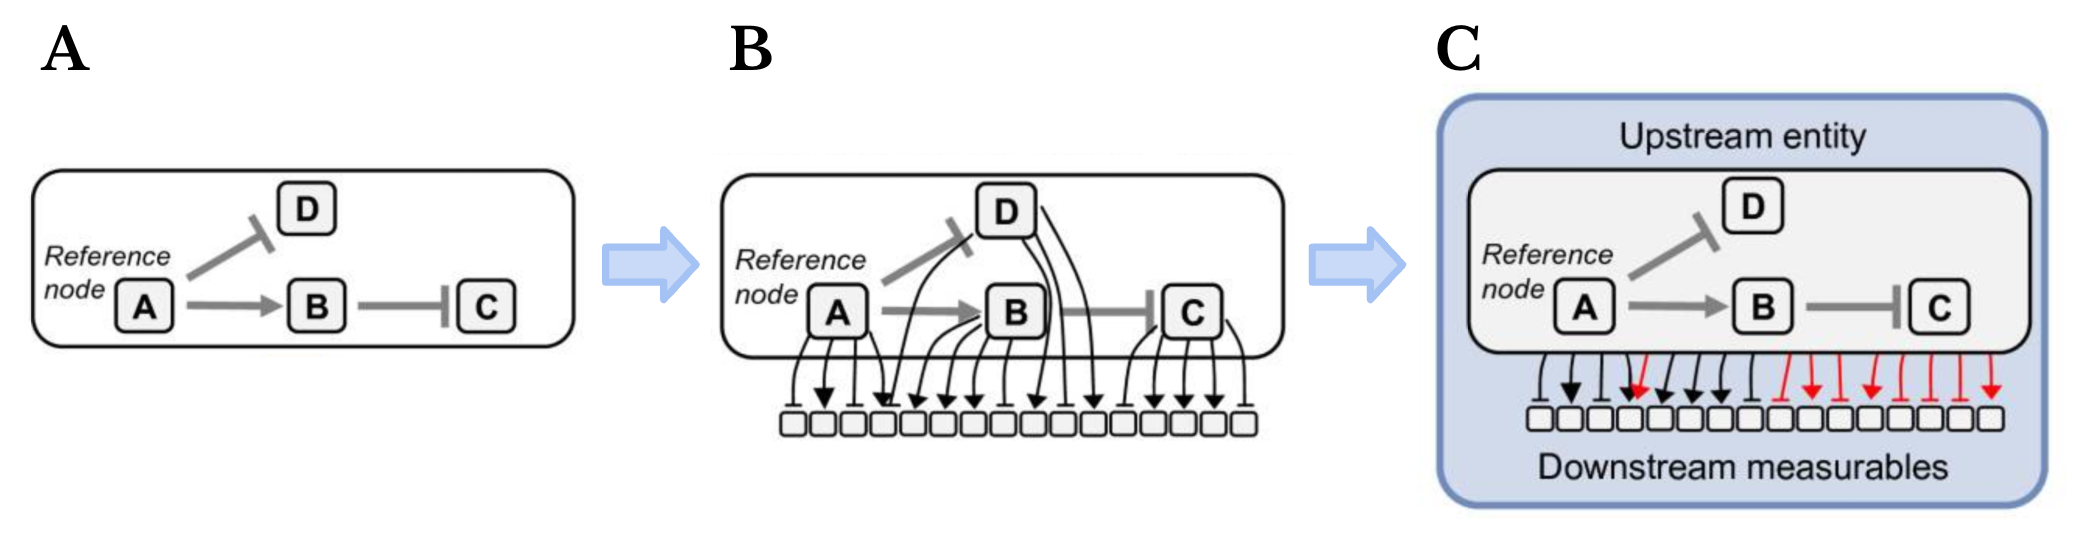
\includegraphics[width=160mm]{figures/npa_schematic.png}}
\caption[Hypothesis Network Generation for Network Perturbation Amplitude]{Creation of hypothesis networks that accounts for the topology and interactions of  upstream controller layer with respect to a reference node A), their individual effects on the downstream layer B) and their combine effect C). Adapted from~\cite{Martin2012}.}
\label{fig:npa_schematic}
\end{figure}

\subsubsection{Sampling of Spanning Trees}

While \ac{NPA} enables more informed analyses than \ac{RCR}, its mathematical basis limits the topologies of knowledge networks that can be used to those with causal consistency.
In these networks, all paths from one node to another result in the same aggregated effect of increases and decreases.
An additional approach in Figure~\ref{fig:sst_schematic} for \ac{SST} with random walkers eliminates inconsistencies and can be aggregated over multiple trials to assign \ac{NPA} scores to networks that were otherwise inconsistent~\cite{Vasilyev2014}.

\begin{figure}
\captionsetup{format=plain}
\makebox[\textwidth]{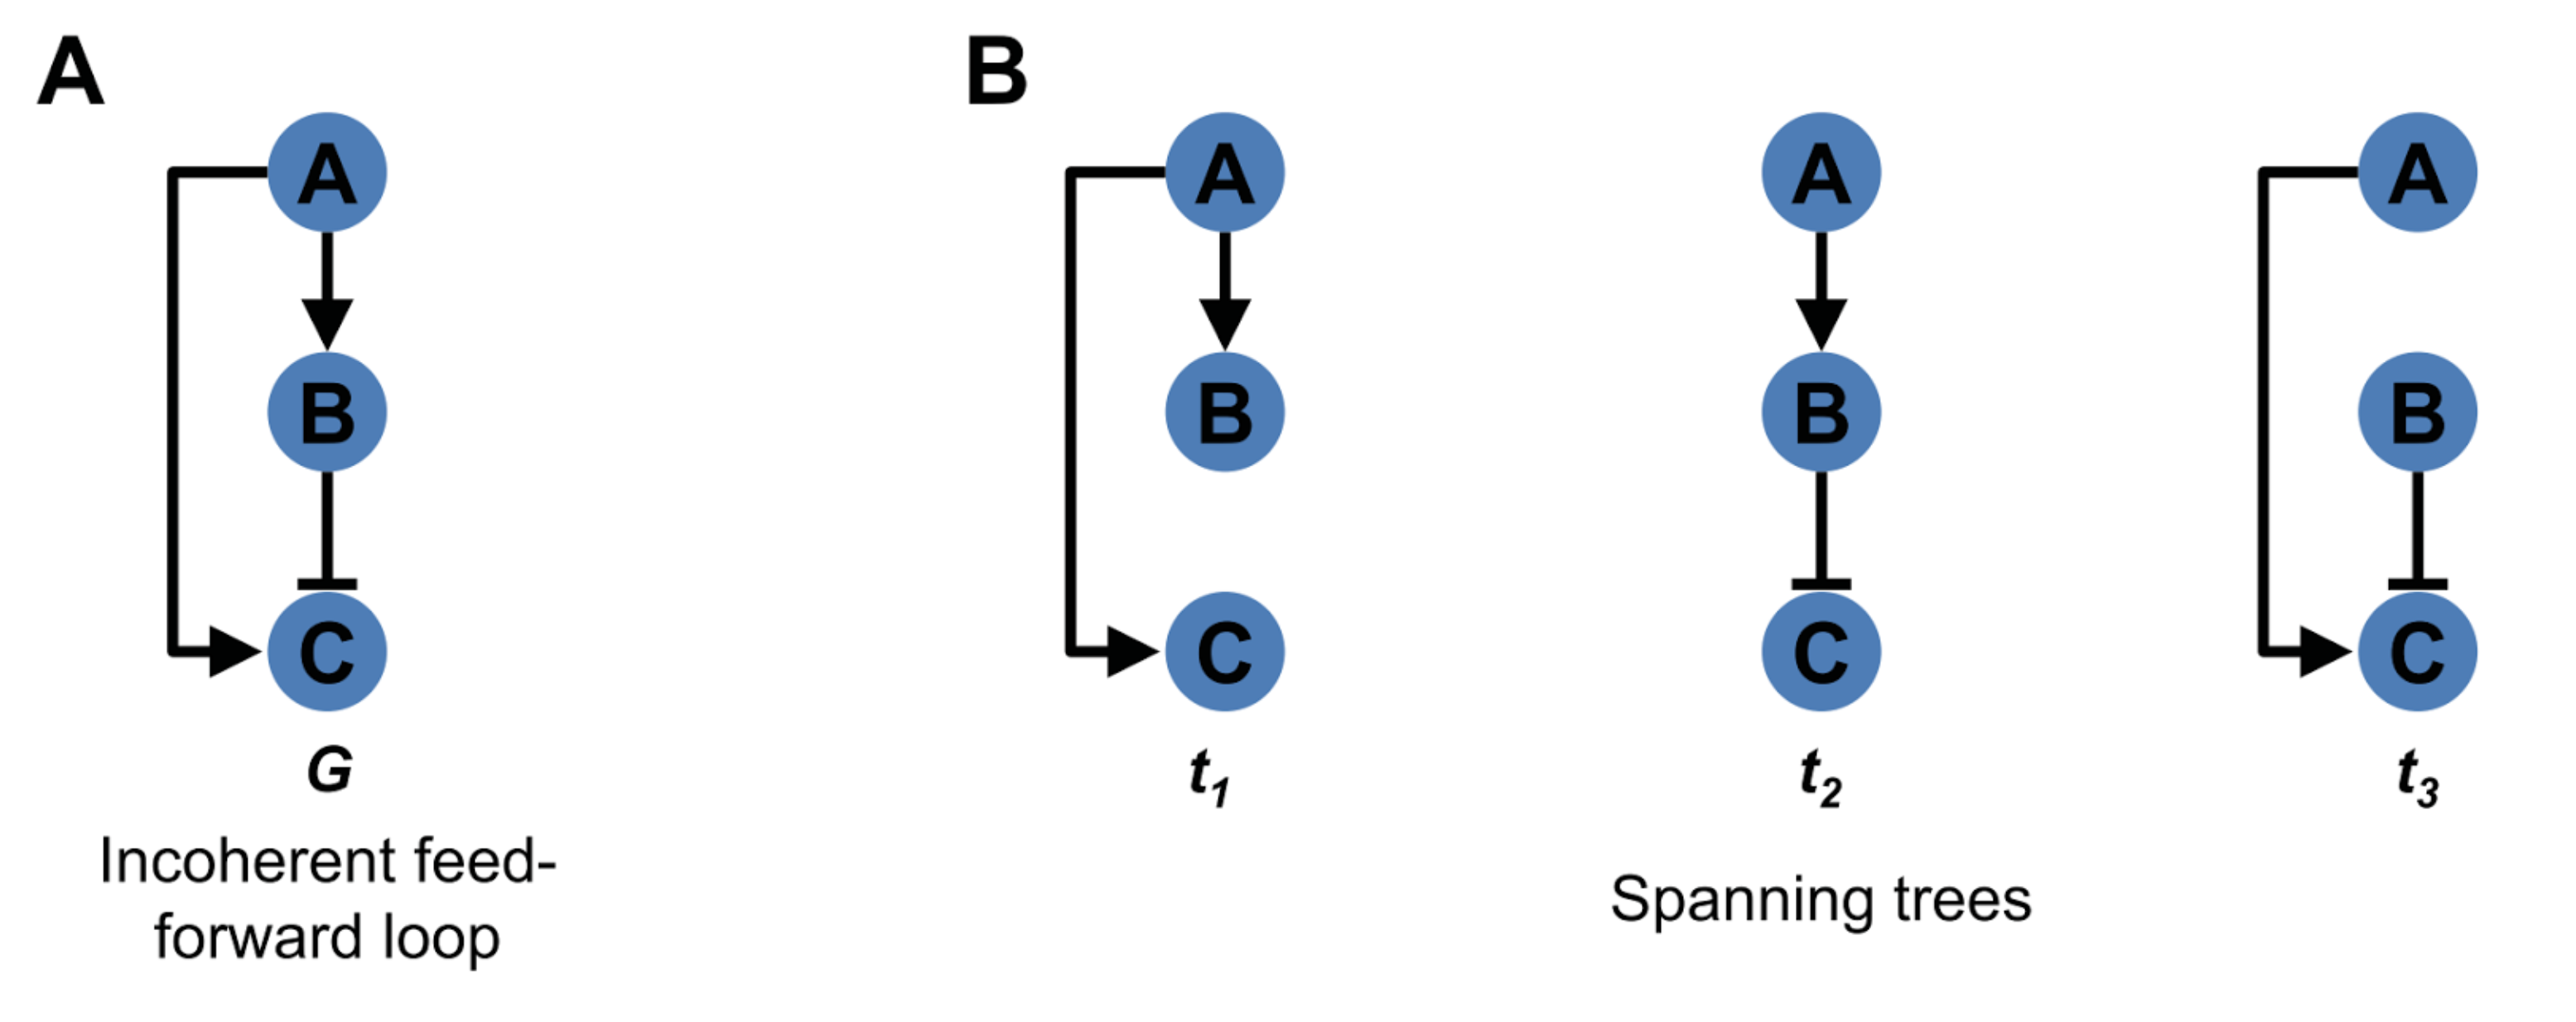
\includegraphics[width=160mm]{figures/sst_example.png}}
\caption[Decomposition of Spanning Trees]{An example decomposition of a small causally inconsistent network A) to its spanning trees B)\cite{Vasilyev2014}.}
\label{fig:sst_schematic}
\end{figure}
